In order to facilitate development we implmemented a full DVS simulator that
generates events from a spherical panorama.  This allows us to develop and test
each part of the algorithm independently with perfect input data and ground
truth. It also makes experimentation easier as everything can be inspected at
will.

The simulation starts off with a normal image containing a 360 degree panorama. The field of view of the camera is computed given its orientation (normal Euler angles) and the panorama image (the ground truth map) is sampled using raycasting. The camera is then rotated by a tiny amount to get a second image patch. These patches are then subtracted to get a list of events.

// TODO insert section to explain camera simulation

\begin{itemize}
\item use image as input
\item assume 360 deg view
\item compute camera fov for given orientation
\item move camera over scene
\item sum up differences between patches
\item problem: discrete
	$\rightarrow$ use tiny steps
		$\rightarrow$ slow
\end{itemize}

\begin{figure}
\label{fig:simulation}
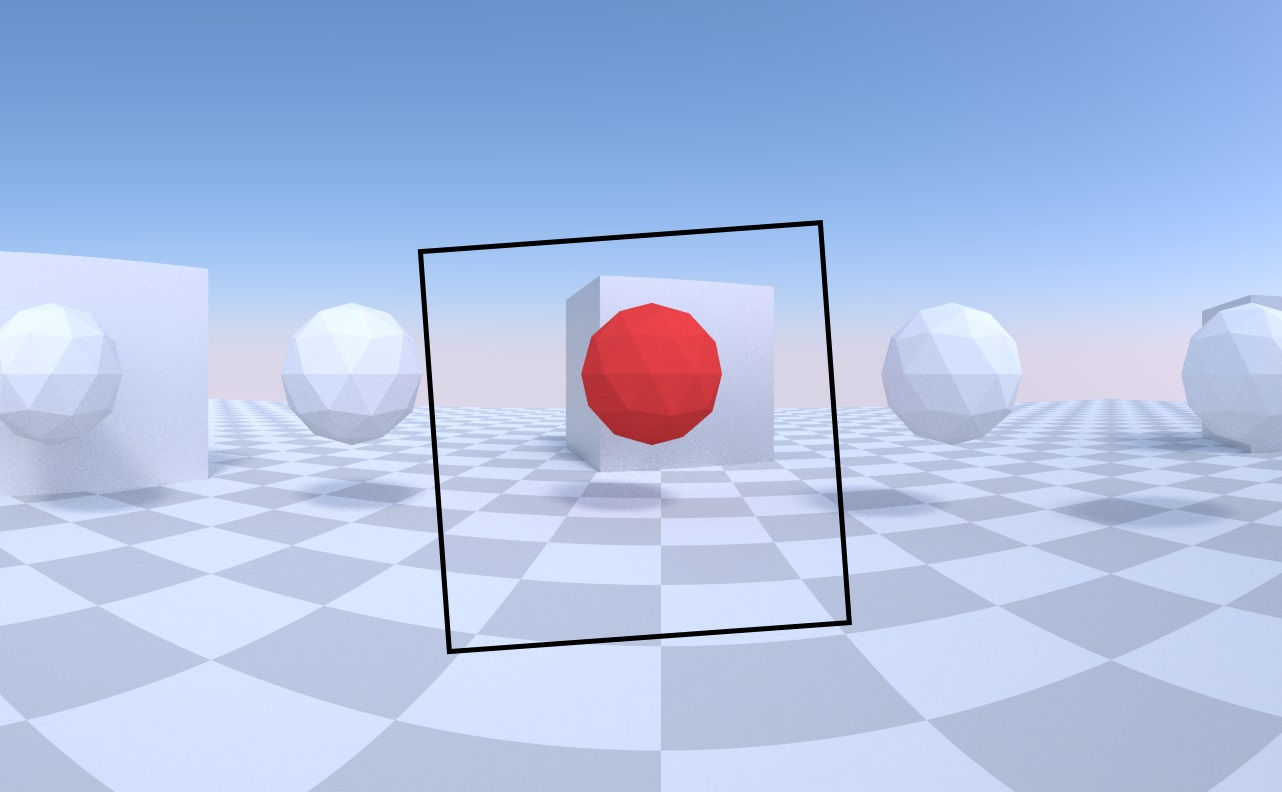
\includegraphics[width=\linewidth]{images/simulation_raw.jpg}
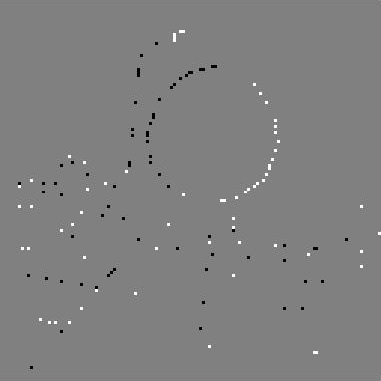
\includegraphics[width=\linewidth]{images/simulation_events.jpg}
\caption{// TODO}
\end{figure}
